\documentclass[a4paperbi]{article}
\usepackage[utf8]{inputenc}
\usepackage[italian]{babel}
\usepackage{titling}
\usepackage{graphicx}
\usepackage{wrapfig}
\usepackage{float}
\usepackage{amsmath}
\usepackage{listings}
\usepackage[table,xcdraw]{xcolor}
\usepackage[numbers]{natbib}
\usepackage{amssymb}
\usepackage[colorinlistoftodos]{todonotes}
\usepackage[LGR,T1]{fontenc}

\renewcommand{\bibfont}{\small}
\newcommand{\textgreek}[1]{\begingroup\fontencoding{LGR}\selectfont#1\endgroup}
\newcommand{\HRule}{\rule{\linewidth}{0.5mm}} % Defines a new command for the horizontal lines, change thickness here

\begin{document}

\begin{titlepage}
\center % Center everything on the page
%----------------------------------------------------------------------------------------
%	HEADING SECTIONS
%----------------------------------------------------------------------------------------
\textsc{\LARGE Università degli studi di}\\[0.1cm]
\textsc{\LARGE Milano-Bicocca}\\[1.2cm] % Name of your university/college
\textsc{\Large Dipartimento di Fisica "G. Occhialini"}\\[0.5cm] % Major heading such as course name
\textsc{\large Tesi di laurea triennale per il corso di Fisica}\\[0.5cm] % Minor heading such as course title
%----------------------------------------------------------------------------------------
%	TITLE SECTION
%----------------------------------------------------------------------------------------
\HRule \\[0.4cm]
{ \huge \bfseries Studio della Stabilità}\\[0.1cm]
{ \huge \bfseries dei Dischi di Accrescimento}\\[0.1cm]
{ \huge \bfseries  di Shakura \& Sunyaev}\\[0.4cm] % Title of your document
\HRule \\[1.5cm]
%----------------------------------------------------------------------------------------
%	AUTHOR SECTION
%----------------------------------------------------------------------------------------
\begin{minipage}{0.4\textwidth}
\begin{flushleft} \large
\emph{Autore:}\\
Riccardo Aurelio \textsc{Gilardi} % Your name
\end{flushleft}
\end{minipage}
~
\begin{minipage}{0.4\textwidth}
\begin{flushright} \large
\emph{Relatore:} \\
Prof. Massimo \textsc{Dotti} % Supervisor's Name
\end{flushright}
\end{minipage}\\[2cm]
%----------------------------------------------------------------------------------------
%	DATE SECTION
%----------------------------------------------------------------------------------------
{\large \today}\\[1cm] % Date, change the \today to a set date if you want to be precise
%----------------------------------------------------------------------------------------
%	LOGO SECTION
%----------------------------------------------------------------------------------------
	\begin{figure}[H]
		\centering
		
\includegraphics[width=0.4\linewidth]{LogoBicocca}
		\label{fig:logobicocca}
	\end{figure} % Include a department/university logo - this will require the graphicx package
%----------------------------------------------------------------------------------------
\vfill % Fill the rest of the page with whitespace
\end{titlepage}

\newpage
\vspace*{\fill}
\textit{Ringraziamenti}\\[2cm]

%\begin{flushright}
%\textit{\textgreek{'o Je`os `ae'i gewmetre\~i}}
%\textit{In realtà un lavoro simile non termina mai.\\Lo si deve considerare concluso quando,\\a seconda del tempo e delle circostanze,\\si è fatto il possibile}\\\textbf{Johann Wolfgang Von Goethe\\Italienische reise (1789)}
%\end{flushright}
\vspace*{\fill}

\newpage
\tableofcontents

\newpage
\section{Introduzione}
Lo scopo di questa tesi vuole essere quello di riassumere ed approfondire le teorie sulla stabilità delle regioni interne dei dischi di accrescimento, nel contesto del modello introdotto da Shakura e Sunyaev nel loro articolo del 1973\footnote{~\cite{ShakuraSunyaev1973}}.

Anche se sarebbe interessante approfondire l'argomento, non considererò il caso dell'accrescimento a simmetria sferica, perché nonostante questo tipo di fenomeno abbia interessato i primi autori che si sono approcciati al tema dell'accrescimento (iniziando dagli studi di Zeldovich negli anni '40, ma continuando con gli studi sviluppatasi in seguito: Salpeter (1964), Lynden-Bell (1969), Schwartzmann (1971) e altri), nella letteratura si è dimostrato come si tratti di un meccanismo troppo poco efficente per essere rilevato, anche nel caso di corpi centrali molto massicci e compatti\footnote{~\cite{PringleReesePacholczyk1973}}.

Per mantenere una descrizione più semplice e meno dispersiva, ho deciso di lavorare seguendo l'esempio di molti autori, analizzando un sistema formato da una stella ordinaria e un buco nero non rotante. Questa scelta è guidata dal fatto che il materiale in accrescimento non risente di effetti legati alla relatività generale a distanze maggiori di tre volte il raggio di Scwartzchild del buco nero
\footnote{Come dimostrato nella sezione 6.7 del ~\cite{FrankKingRaineAccretionPower}}
e, al contrario del caso di accrescimento intorno a una stella a neutroni, il sistema in accrescimento al buco nero non sarà interessato da fenomeni legati ai campi magnetici e alla torsione che essi possono applicare al materiale in accrescimento.

La scelta è anche giustificata dal fatto che, nonostante i buchi neri che fanno parte di sistemi binari siano meno semplici da osservare rispetto, per esempio, di quelli contenenti nane bianche, la loro estrema compattezza permette di apprezzare il comportamento del disco nelle sue regioni più interne.

Prima di parlare delle instabilità nei dischi, comincerò introducendo i concetti e le formule che descrivono un disco di accrescimento sottile, la fisica che ne governa lo stato stazionario e il meccanismo con cui si può arrivare alla formazione.

\newpage
\section{Accrescimento in sistemi binari}
	L'accrescimento è uno dei processi di conversione di massa in energia tra i più efficienti nell'universo, che si sviluppa in sistemi binari di cui almeno un membro è un corpo compatto: una nana bianca, una stella a neutroni o un buco nero.

	Tra le cause scatenanti del trasporto di materiale tra due membri di un sistema binario, sono particolarmente importanti il travalicamento da parte di uno dei membri del sistema del suo lobo di Roche o la cattura gravitazionale da parte del corpo compatto di venti stellari emessi dal suo compagno. Il primo di questi due processi è sicuramente meglio descritto e più semplice da trattare analiticamente e permette di dedurre delle informazioni interessanti sul processo dissipativo che permette il trasporto del momento angolare. Una descrizione di questi processi permette di definire al meglio le ipotesi su cui si costruiscono i modelli di disco di accrescimento e permettono di fare osservazioni quantitative interessanti.
	
	Comunque è interessante sapere che la perdita di materiale tramite venti è molto comune e particolarmente importante quando l'accrescimento avviene con tassi superiori a quelli imposti dal limite di Eddington.
	
	\begin{equation}
		\dot{M}=\frac{4\pi GMm_pc^3}{\sigma_T \eta}
	\end{equation}

\subsection{Deflusso attraverso i Lobi di Roche}
	Edouard Roche ricavò la forma della struttura che ora prende il suo nome studiando l'orbita dei satelliti planetari. Lo fece descrivendo il moto di alcune particelle di test immerse in un potenziale gravitazionale generato da due corpi orbitanti intorno alla loro reciproca attrazione gravitazionale.
	
	La sua costruzione è essenziale e piuttosto elegante e si può ricavare partendo da poche semplici ipotesi, prima di calcolarne numericamente i parametri: la particella di test deve avere massa abbastanza piccola, al confronto con quella dei due corpi massicci, da non poterne influenzare in modo rilevante l'orbita; le orbite sono da considerarsi kepleriane e circolari, questo non è sempre vero in pratica, ma in generale le forze mareali tendono a rendere circolari orbite eccentriche in tempi scala molto minori di quelli caratteristici di un meccanismo di trasporto di materia; infine le masse sono da considerarsi condensate nel loro centro.
	
	Per descrivere qualsiasi flusso di gas tra i due corpi del sistema ha senso scrivere l'\textit{equazione di Eulero} in un sistema di riferimento co-rotante col sistema binario, con velocità angolare $\omega$ rispetto al sistema inerziale. Questo comporta la presenza nell'equazione di termini che tengano conto delle forze centrifughe e di quelle di Coriolis ($-2\omega\times\textbf{v}$), così che diventa:
	\begin{equation}
		\frac{\partial \textbf{v}}{\partial t}+(\textbf{v}\cdot\nabla)\textbf{v}=-\nabla\Phi_R-2\omega\times\textbf{v}-\frac{1}{\rho}\nabla P
	\end{equation}
	Con $\omega$ parallela al versore ortogonale al piano orbitale $\textbf{e}$:
	\begin{equation}
		\omega=\left[\frac{G(M_1+M_2)M_\odot}{a^3}\right]^{1/2}\textbf{e}
	\end{equation}
	e $\Phi_R$ il \textit{Potenziale di Roche}\footnote{Immagine da ~\cite{FrankKingRaineAccretionPower}}, che contiene i termini relativi all'attrazione gravitazionale e le forze centrifughe (ma non quelli relativi a Coriolis):
	\begin{equation}
		\Phi_R(\textbf{r})=-\frac{GM_1M_\odot}{\vert\textbf{r}-\textbf{r}_1\vert}-\frac{GM_2M_\odot}{\vert\textbf{r}-\textbf{r}_2\vert}-\frac{1}{2}(\omega\times\textbf{r})^2
	\end{equation}
	
	\begin{figure}[H]
		\centering
		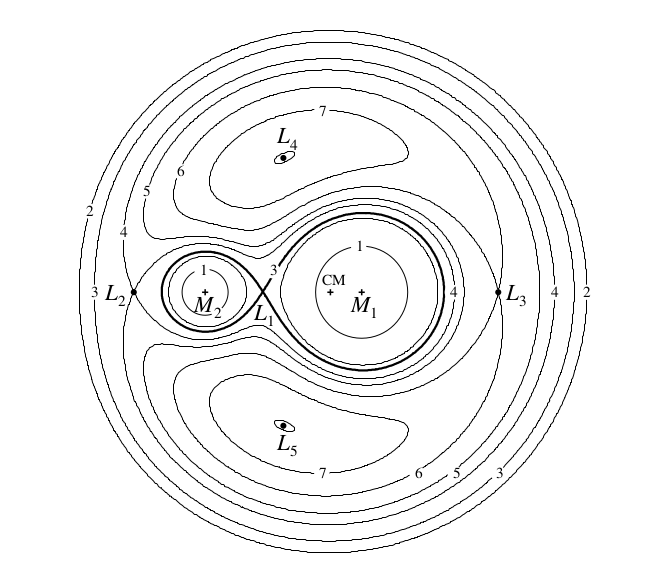
\includegraphics[width=0.6\linewidth]{RocheEquipotential}
		\caption{Una rappresentazione della sezione dei lobi e delle curve equipotenziali di $\Phi_R$. $L_1$ è il punto lagrangiano interno.}
		\label{fig:rocheequipotential}
	\end{figure}
	
	Le curve equipotenziali di $\Phi_R$ dipendono solo dal rapporto fra le masse $q=\frac{M_2}{M_1}$ e la loro scala dipende dalla distanza che le separa, $a$. Per $q\sim1$ i lobi saranno simmetrici, mentre per rapporti $q\ll1$ o $q>>1$ avranno volumi diversi.
	
	Per distanze sufficientemente alte, la forma delle curve equipotenziali corrisponde a quella di una singola massa $M=(M_1+M_2)M_\odot$, mentre a distanze brevi il potenziale è dominato da quello della stella più vicina. Le buche di potenziale centrate sulle posizioni dei due corpi $\textbf{r}_1$ e $\textbf{r}_2$, sono separate dalla cosiddetta \textit{superficie critica}.
	
	Il punto separatore dei due lobi, detto \textit{punto lagrangiano interno} è una sella per $\Phi_R$ tale che se del materiale in uno dei due lobi si trovasse in sua prossimità (magari a seguito dell'espansione della stella da cui proviene, che si ritroverà ad occupare tutto il volume del suo lobo), passerebbe attraverso lui verso il lobo della compagna, piuttosto che attraversare la superficie critica del potenziale.
	
	Si può trattare in maniera quantitativa la stima della geometria dei lobi e sul trasporto di materia, ricavando quindi la loro dipendenza da $q$ ed $a$. Qualcosa che è interessante osservare è che questi due termini varieranno nel tempo durante qualsiasi processo di accrescimento, comportando una contrazione del lobo del corpo che sta cedendo massa ed una riduzione del periodo orbitale del sistema, insieme alla riduzione della distanza tra i due corpi, dovuta al processo di trasferimento del momento angolare nel sistema.
	
	Si può dimostrare che, nell'ipotesi di accrescimento lento e totale $\dot{M}_1+\dot{M}_2=0$, il trasferimento di materia tra i due lobi si svolge nello stesso tempo scala con cui il momento angolare viene perso.
	
	Ipotizzando sia $M_2$, che chiameremo stella secondaria, a cedere materia a $M_1$, il nostro buco nero o primaria. Con $J$ momento angolare totale del sistema, abbiamo che:
	
	\begin{equation}
		-\frac{\dot{M}_2}{M_2}=\frac{-\dot{J}/J}{4/3-M_2/M_1}
	\end{equation}
	
	e analogamente si trova che

	\begin{equation}
		\frac{\dot{a}}{a}=2\frac{\dot{P}}{3P}=\frac{2\dot{J}/3J}{4/3-q}
	\end{equation}
	
\subsection{Formazione di un disco}
	Il trasporto di materia attraverso i lobi ne aumenta anche il momento angolare in quantità non indifferente, tanto da non permettere al materiale di essere accresciuto direttamente alla primaria, senza che qualche meccanismo gliene faccia trasportare la maggior parte.
	
	Se il periodo orbitale del sistema non è molto lungo, il lobo primario, ovvero quello a cui viene accresciuta la materia, la vedrà provenire dal punto lagrangiano con velocità quasi completamente ortogonale alla linea dei centri, che unisce le due masse. 
	
	Se definisco $b_1$ la distanza tra $M_1$ e $L_1$, posso approssimare il valore della componente istantaneamente ortogonale alla linea dei centri della velocità in un sistema di riferimento inerziale con
	\begin{equation}
		v_\perp\sim b_1\omega\sim 100\,M_1^{1/3}(1+q)^{1/3}P^{-1/3}_{day}\,km\,sec^{-1}
	\end{equation}  
	Mentre per la componente parallela, poiché immagino la forza che permette il passaggio tra i lobi della materia sia legata alla pressione, posso supporre valga
	\begin{equation}
		v_\parallel \lesssim c_{s}
	\end{equation}
	con $c_{s}$ velocità del suono nel lobo secondario, da cui proviene la materia. Poiché nel mezzo interstellare la temperatura ha valori $T\lesssim10^5\,K$ e poiché in generale per un gas vale $c_s\cong10(T/10^4\,K)^{1/2}km\,sec^{-1}$, deve essere $v_\parallel\lesssim10\,km\,sec^{-1}$
	
	Quindi in totale il moto del gas in ingresso al lobo primario deve essere supersonico. Questa condizione viene poi rinforzata dall'accelerazione che il materiale in accrescimento subirà per l'azione del campo gravitazionale del buco nero.

	\paragraph{Orbita del gas}	
	Si può dimostrare come le forze di pressione abbiano un effetto trascurabile sul materiale, che quindi si muoverà con orbita ballistica nel potenziale di Roche del corpo a cui sta accrescendo, come una particella di test. Inoltre il suo moto ellittico subirà una precessione dovuta all'effetto della presenza del corpo da cui proviene.
	
	Poiché $v_\parallel\sim c_s$ è molto minore delle velocità di free-fall che le particelle acquisirebbero nell'avvicinamento a $M_1$, le condizioni iniziale all'attraversamento di $L_1$ hanno un effetto praticamente irrilevante sulla loro orbita, che sarà quindi essenzialmente unica per ogni particella di test. Queste orbite dovranno comunque intersecarsi fra loro per via della precessione a cui sono soggette tutte singolarmente. Per un flusso continuo di gas, questo comporta la dissipazione di energia termica tramite degli urti (\textit{shock}) fra le particelle che lo formano. 
	
	Attraversato $L_1$, il gas in accrescimento si troverebbe, senza un meccanismo di dissipazione, a seguire l'orbita a potenziale minore per un dato momento angolare ($R_{circ}v_\phi(R_{circ})=b_1^2\omega$), ovvero un'orbita circolare, ad un certo raggio $R_{circ}$ e con velocità circolare
	\begin{equation}
		v_\phi(R_{circ})=\left(\frac{GM_1M_\odot}{R_{circ}}\right)^{1/2}
	\end{equation}
	
	E' possibile ricavare il valore del \textit{raggio di circolarizzazione} $R_{circ}$, utilizzando la formula del periodo della binaria $\omega=2\pi/P$ e si può dimostrare tramite la computazione dei parametri dei lobi come questo sia di un fattore $2\sim3$ più piccolo del raggio medio del lobo primario. Questo comporta che, a meno del caso in cui il raggio della primaria sia maggiore del raggio di circolarizzazione ($R_\star>R_{circ}$), la materia tenderebbe ad orbitare stabilmente nel lobo, una volta superata $L_1$.
	Non risulta interessante considerare l'eccezione sopracitata, poiché l'accrescimento è un processo tanto più efficente tanto più sono compatti gli oggetti intorno a cui avviene e se per una nana bianca realisticamente $R_{WD}\lesssim10^9\,cm$ normalmente ci si aspetta per il raggio di circularizzazione un valore $R_{circ}\gtrsim3.5\times10^9P_{hr}^{2/3}\,cm$.

	Un anello di materia dovrà necessariamente subire dei processi dissipativi, come degli urti, che convertiranno necessariamente parte dell'energia del moto orbitale delle particelle che lo formano in energia interna, ovvero calore. Parte di questa energia sarà irradiato, con una certa efficenza $\eta$ e quindi perso dal gas, costringendo le sue particelle interessate dalla dissipazione ad avvicinarsi alla primaria (nell'ipotesi in cui risentano del solo potenzile gravitazionale del corpo massiccio). 
	Affinché sia conservato il momento angolare nel disco, parte del momento delle particelle che si stanno avvicinando al corpo massiccio dovrà essere trasportato verso l'esterno. Il tempo di redistribuzione del momento angolare è maggiore sia dei tempi scala di raffreddamento radiativo $t_{rad}$ che di quello orbitale (dinamico) $t_{din}$. Quindi parte del gas che orbitava sul raggio di circularizzazione, perdendo energia e trasportando momento angolare, spiraleggerà lentamente verso la primaria, costretto in una serie di orbite approssimamente circolari, nella configurazione cosiddetta di \textbf{disco di accrescimento}. 	
	
	In assenza di torsioni esterne, mi aspetto che le particelle esterne del disco, a cui viene trasferito momento, debbano spiraleggiare verso l'esterno a raggi maggiori di quelli di circularizzazione, fino a a una distanza tale per cui qualche meccanismo non gli impedisca di allontanarsi oltre\footnote{In realtà poiché il \textit{momento angolare specifico} $h$ per materia che orbita ad un raggio $R$ vale $h=R^2\Omega\propto R^{1/2}$ e quindi tende all'inifinito per raggi infiniti, la materia tenderà definitivamente a dirigersi verso il centro del disco, con il momento che tenderà ad allontanarsi a distanze sempre maggiori.}.
		
\subsection{Processi Dissipativi}
	Per un elemento di gas di massa $m$, che stia raggiungendo l'ultima orbita stabile (Innermost Stable Circular Orbit) intorno al buco nero, l'energia di legame varrà $E=\frac{1}{2}\frac{GMm}{R_\star}$. Considerando il valore di questa energia come trascurabile alla distanza da cui provengono, posso dire che la luminosità totale del disco dovrà valere
	
	\begin{equation}
		L_{disc}=\frac{GM\dot{M}}{2R_\star}=\frac{1}{2}L_{acc}
	\end{equation}

	Questo comporta che se metà dell'energia viene irradiata dalla materia che si muove verso l'ISCO, l'altra metà dovrà essere irradiata tutta nelle regioni prossime al bordo interno del disco. Inoltre se considero che il momento angolare per raggio vale $R^2\Omega(R)\propto R^{1/2}$ e che $R_{ISCO}\ll R_{circ}$, il gas che forma il disco dovrà perdere quasi completamente il suo momento nella discesa verso la primaria.
	
	Nel contesto dei dischi di accrescimento, strutture gassose con una rotazione differenziale rispetto al raggio formate di particelle con velocità circa ortogonale alla direzione radiale, posso supporre che il meccanismo di trasporto del momento angolare e di dissipazione dell'energia in calore sia legato alla \textit{tensione viscosa di taglio} che si esercita fra strati diversi del disco.
	
	Si può capire come avvenga il trasporto di momento angolare per dissipazione viscosa considerando per esempio due strati successivi del disco di uno spessore arbitrariamente piccolo $\lambda$, separate da una superficie a che si trova a distanza $R$ dal centro del buco nero. Elementi del fluido che forma il disco, muovendosi caoticamente, potranno continuamente venire scambiati tra i due strati con velocità $\tilde{v}$. Questi elementi percorreranno in media una distanza $\lambda$ prima di interagire con elementi dello strato che hanno raggiunto e poiché la loro velocità dipendeva dal raggio a cui sono partiti, dopo una serie di scambi, ci sarà un \textit{trasporto netto di momento angolare} tra i due strati. Questo senza un trasporto netto di materia, per simmetria.
	
	\paragraph{Forma della viscosità}	
	Al momento non siamo ancora in grado di dare prescrizioni fisiche per la stima dei valori di $\lambda$ e $\tilde{v}$, così strettamente legati al significato fisico della dissipazione viscosa che agisce nel disco. Risultati moderni collegano la viscosità a processi magnetici, come suggerito da Balbus e Hawley nel 1991, ma non esiste ancora una risposta certa o esaustiva a riguardo. 
	
	Si dimostra che in generale la densità di forza viscosa di taglio vale
	\begin{equation}
		f_{visc,taglio}\sim\rho\lambda\tilde{v}\frac{\partial^2v_\phi}{\partial R^2}\sim\rho\lambda\tilde{v}\frac{v_\phi}{R^2}
	\end{equation}
	Questo ci permette di ricavare un valore per il \textit{termine di Reynolds}, che stima l'importanza dinamica del termine viscoso rispetto a quello inerziale (ovvero $\rho(\partial\textbf{v}/\partial t+(\textbf{v}\cdot\nabla)\textbf{v})$, estratto dall'equazione di Eulero)
	\begin{equation}
		Re\sim\frac{v_\phi^2/R}{\lambda\tilde{v}v_\phi/R^2}=\frac{Rv_\phi}{\lambda\tilde{v}}
	\end{equation}
	Quindi possiamo dimostrare che la viscosità che permette l'accrescimento non è semplicemente quella classicamente legata ad un gas, per cui sarebbero $\lambda\sim\lambda_d$ \textit{tempo di deflessione} delle particelle del gas e $\tilde{v}\sim c_s$ velocità del suono, poiché in questo caso, utilizzando risultati della fluidodinamica, troviamo che sarebbe $Re_{mol}\gtrsim10^4$ in regioni interne a un tipico disco di accrescimento. Questo valore iplicherebbe una irrilevanza estrema del termine viscoso rispetto a quello inerziale nel disco, dimostrando che la "viscosità molecolare" non può essere responsabile del trasporto.
	
	Poiché si è dimostrata sperimentalmente l'esistenza di un \textit{numero di Reynold critico} oltre cui il moto del gas diventa turbolento, con grandi variazioni di velocità in grande e piccola scala, si potrebbe supporre che anche nei dischi di accrescimento il processo principale di redistribuzione del momento angolare sia un moto turbolento, anche se non è stato dimostrato.
	La viscosità in questo tipo di sistema dipenderebbe da una lunghezza caratteristica dei vortici pi grandi, che ci aspettiamo non poter superare l'altezza del disco $\lambda_{turb}\lesssim H$ e da una velocità degli stessi vortici che ci aspettiamo essere subsonica $v_{turb}\lesssim c_s$, tali per cui $\nu_{turb}\sim \lambda_{turb}v_{turb}$.
	Poiché non siamo ancora in grado di descrivere matematicamente un moto turbolento, né capiamo appieno i meccanismi fisici che ne regolerebbero l'intesità, si è dimostrato utile, in un approccio semi-empirico all'analisi dei dischi, parametrizzare la viscosità con
	\begin{equation}
		\nu=\alpha c_s H
	\end{equation}
	Questa è la cosiddetta \textit{condizione $\alpha$ di Shakura e Sunyaev}, con $\alpha\lesssim 1$ adimensionale: una parametrizzazione utile per la costruzione di un modello di disco, che riesce a sintetizzare la nostra ignoranza sulla natura della viscosità, che non ci permette di avere un modello deterministico di disco.

	\paragraph{Momento torcente ed energia dissipata}
	Una frazione di fluido dallo strato più interno trasporterà in media un momento $L(R+\lambda/2)$, mentre una dallo strato più esterno trasporterà in media $L(R-\lambda/2)$. Questo trasporto netto si traduce in una \textit{torsione del disco interno su quello esterno}.
	
	Se i due strati hanno densità $\rho(R)$ e altezza $H(R)$, ci sarà un trasporto di materia netto nell'ordine di $H\rho\tilde{v}$ e per un osservatore co-rotante con il fluido che si trovi sulla superficie di separazione il \textit{momento torcente medio} che si esercitano reciprocamente per unità di angolo e al primo ordine in $\lambda$ varrebbe:
	\begin{equation*}
		-\rho\tilde{v} H\lambda R^2\frac{d\Omega}{dr}
	\end{equation*}
	E per il nostro sistema di dischi concentrici, definendo la \textit{densità superficiale} $\Sigma=H\rho$ e il \textit{coefficente di viscosità cinematica} $\nu\sim\lambda\tilde{v}$, possiamo scrivere il \textit{momento torcente} esercitato dal disco esterno su quello interno come
	\begin{equation}
		G(R)=2\pi R\nu\Sigma R^2\frac{d\Omega}{dr}
	\end{equation}
	Si può apprezzare l'efficacia di questa formula nel descrivere l'accrescimento notando come si annulla nel caso di una rotazione rigida $\Omega'=\frac{d\Omega}{dr}=0$ ed è negativa nel caso in cui la velocità angolare decresca allontanandosi dal centro del disco, comportando quindi il trasporto del momento angolare dagli strati più interni verso quelli più esterni, con il conseguente spiraleggiare verso l'interno del gas.
		
	Sempre con l'analogia dell'attrito viscoso fra gli strati del disco, si può ricavare una formula per la \textit{frazione di energia dissipata} per unità di area:
	\begin{equation}
		D(R)=\frac{G\Sigma'}{4\pi R}=\frac{1}{2}\nu\Sigma(R\Omega')^2
	\end{equation}
	Funzione sempre positiva o nulla, nel caso della rotazione rigida, legata ovviamente all'efficacia radiativa $\eta$ del nostro sistema.
	
	La formula di $D(R)$ si ricava considerando i due momenti torcenti che agiscono ai due lati di un anello di gas che si estende tra $R$ e $R+dR$, tali per cui, se vengono divisi per la velocità angolare
	\begin{equation}
		\frac{1}{\Omega}(G(R+dR)-G(R))=\frac{1}{\Omega}\frac{\partial G}{\partial R}dR=\frac{1}{\Omega}\left[\frac{\partial}{\partial R}(G\Omega)-G\Omega'\right]dR
	\end{equation}
	Quest'equazione è formata da due termini, primo dei quali è $\frac{\partial}{\partial R}(G\Omega)dR$, che rappresenta il tasso di "spostamento" dell'energia nel gas per mezzo dei momenti torcenti e se integrato per tutti i raggi ha un valore che dipende solo dalle condizioni agli estremi del disco. Il secondo termine è $-G\Omega'dR$ e rappresenta un tasso di perdita locale di energia meccanica nel gas, che sarà quindi dissipata sotto forma di calore.
	
	La formula di $D(R)$ si ricava considerando che il calore sarà irradiato su entrambe le facce del disco, con superficie $4\pi RdR$.

\newpage
\section{Modello di Struttura del Disco} 	
	Definite le condizioni in cui avviene l'accrescimento e che portano alla formazione intorno al buco nero di un disco, se ne possono descrivere le proprietà e la struttura locale partendo dall'assunzione che sia \textit{sottile}, ovvero considerare il gas che forma il disco così strettamente confinato al piano orbitale che si può trattare come un flusso di materia quasi-bidimensionale. Questa proprietà si può anche riassumere dicendo che ci aspettiamo l'altezza del disco sia ovunque molto minore del suo raggio esterno: $H\simeq\frac{c_s}{v_\phi}R\ll R$, con $v_\phi=\left(\frac{GM}{R}\right)^{1/2}$ velocità kepleriana a distanza $R$ dal buco nero di massa $M$.
	
	Nel loro articolo seminale del 1973 \footnote{~\cite{ShakuraSunyaev1973}}, Shakura e Sunyaev sono stati in grado di dimostrare come l'ipotesi di disco sottile sia precisamente equivalente a quella di raffreddamento efficiente e di orbite kepleriane, così che se una di queste manca, lo fanno tutte. Quindi si dimostra che nelle zone termicamente stabili del disco deve valere l'ipotesi di sottigliezza.
	
	Nell'ipotesi che il materiale del disco orbiti in modo circa kepleriano, posso descrivere il suo spostamento verso il corpo in accrescimento sommando alle velocità kepleriane una componente radiale $v_R$, negativa in un sistema di riferimento centrato su $M$ in coordinate polari.
	
	\paragraph{Conservazione della massa e Densità superficiale}
	Considerando ancora un anello di gas da $R$ a $R+dR$, la cui massa vale $2\pi RdR\Sigma$ e che ha momento angolare totale $2\pi RdR\Sigma R^2\Omega$, il flusso netto tra anelli vicini è descritto dalla variazione di queste due quantità. 
	
	Per la massa
	\begin{gather*}
		\frac{\partial}{\partial R}(2\pi RdR\Sigma)=v_R(R,t)2\pi R\Sigma(R,t)-v_R(R+dR,t)2\pi(R+dR)\Sigma(R+dR,t)\\
		\cong-2\pi dR\frac{\partial}{\partial R}(R\Sigma v_R)
	\end{gather*}
	Che nel limite $dR\rightarrow 0$ è l'\textit{equazione di conservazione della massa} nel disco
	\begin{equation}
		R\frac{\partial\Sigma}{\partial t}+\frac{\partial}{\partial R}(R\Sigma v_R)=0
	\end{equation}
	Analogamente partendo da
	\begin{equation*}
		\frac{\partial}{\partial R}(2\pi RdR\Sigma R^2\Sigma)\cong-2\pi dR\frac{\partial}{\partial R}(R\Sigma v_R R^2\Sigma)+\frac{\partial G}{\partial R}dR	
	\end{equation*}
	Trovo che nel limite $dR\rightarrow 0$ diventa \textit{l'equazione di conservazione del momento angolare nel disco}
	\begin{equation}
		R\frac{\partial}{\partial t}(\Sigma R^2\Omega)+\frac{\partial}{\partial R}(R\Sigma v_R\cdot R^2\Omega)=\frac{1}{2\pi}\frac{\partial G}{\partial R}
	\end{equation}
	Usando la definizione di $G(R)$ e della velocità angolare in un'orbita kepleriana $\Omega_K$,  questa ci permette di definire un'equazione differenziale di $\Sigma$ ed $R$
	\begin{equation}
		\frac{\partial\Sigma}{\partial t}=3R^{-1}\frac{\partial}{\partial R}\left\{R^{1/2}\frac{\partial}{\partial R}\left[\nu\Sigma R^{1/2}\right]\right\}
	\end{equation}
	In generale, supponendo $\nu$ sia una funzione delle condizioni locali del disco (ovvero di $\Sigma$, $R$ e $t$), questa rappresenta un'equazione non lineare di diffusione di $\Sigma$, ma supponendo che $\nu$ sia funzione del solo raggio e scali come una sua potenza, l'equazione diventa lineare e risolvibile analiticamente. In particolare nel caso in cui $\nu$ sia costante, come assunto nel modello di Shakura-Sunyaev, la soluzione per un disco che va da $R=0$ a $R=\infty$ e momento torcente nullo all'origine è
	\begin{equation}
		\Sigma(R,t)=(12)^{1/4}R^{-3/4}\nu^{-3/4}\int^{\infty}_0d\lambda\,f(\lambda)e^{-\lambda^2t}J_{1/4}(R\lambda/\sqrt{3\nu})(R\lambda/\sqrt{3\nu})^{1/4}
	\end{equation}
	Dove $f(\lambda)$ è una funzione che dipende dalle condizioni iniziali e $J_{1/4}$ è la funzione ordinaria di Bessel di ordine $1/4$.
	
	La soluzione corrispondente alla distribuzione iniziale di materia sul disco è l'\textit{equazione di Green} per un anello di massa $m$ che si trovava inizialmente ad un raggio $R_0$, che mi aspetto essere intorno a $R_{circ}$
	\begin{equation}
		\Sigma(R,t=0)=\frac{m}{2\pi R_0}\delta(R-R_0)
	\end{equation}
	
	Posso scrivere questa soluzione implicitamente, definendo i due parametri adimensionali $\chi=R/R_0$ e $\tau=12\nu tR_0^{-2}$, come funzione di $\chi$ per diversi $\tau$:
	\begin{equation}
	\Sigma(\chi,\tau)=\frac{m}{\pi R_0^2}\tau^{-1}\chi^{-1/4}exp\left\{-\frac{1+x^2}{\tau}\right\}I_{1/4}(2\chi/\tau)
	\end{equation}
	$I_{1/4}$ è la funzione di Bessel modificata.
	
	Ponendo $(1+\chi^2)\tau^{-1}\sim 1$, questa equazione ci mostra come la viscosità influenzi la densità superficiale originale in un \textit{tempo scala viscoso} o \textit{di scivolamento radiale} $t_{visc}\sim R^2/\nu$ e anche che $\tau\sim t/t_{visc}(R_0)$.
	
	Il tempo scala si può chiamare di "scivolamento radiale", perché l'equazione usata per derivare $\frac{\partial\Sigma}{\partial t}$ permette anche di derivare una funzione per le velocità radiali
	\begin{equation}
		v_R=-\frac{3}{\Sigma R^{1/2}}\frac{\partial}{\partial R}(\nu\Sigma R^{1/2})
	\end{equation}
	Tale per cui $v_R\sim\frac{\nu}{R}\sim\frac{R}{t_{visc}}$.
	
	Costruendo un grafico della densità di superficie nel tempo\footnote{Immagine da ~\cite{Pringle1981}} si può notare come questa si evolva dall'anello ad $R_0\sim R_{circ}$ in una distribuzione asimmetrica, più alta verso il centro del disco che verso il suo esterno, dove comunque parte della materia si dirige per la conservazione del momento angolare totale.
	
	\begin{figure}[H]
		\centering
		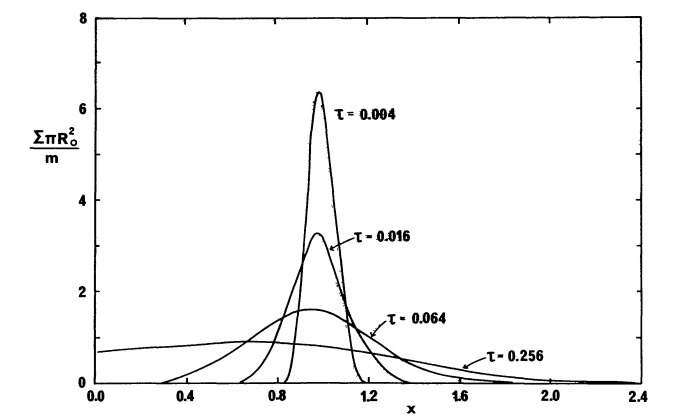
\includegraphics[width=0.7\linewidth]{DensSuper}
		\caption{Evoluzione viscosa di un disco di materia di massa $m$ in funzione di $x=R/R_{circ}$, con $\tau=12\nu t/R_{circ}^2$.}
		\label{fig:denssuper}
	\end{figure}

	Questo risultato è reso evidente analiticamente se si considera che, poiché il comportamento asintotico dell'equazione modificata di Bessel è
	\begin{equation*}
		I_{1/4}(z)\propto\begin{cases}
				z^{-1/2}e^z\text{ per $z\gg1$}\\
				z^{1/4}\text{ per $z\gg1$}
			\end{cases}
	\end{equation*}	 
	allora per la velocità radiale dovrà valere
	\begin{equation*}
		v_R\sim\begin{cases}
			\frac{3\nu}{R_0}\left\{\frac{1}{4\chi}+\frac{2\chi}{\tau}-\frac{2}{\tau}\right\}\text{ per $2\chi\gg\tau$}\\
			-\frac{3\nu}{R_0}\left\{\frac{1}{2\chi}-\frac{2\chi}{\tau}\right\}\text{ per $2\chi\ll\tau$}			
			\end{cases}
	\end{equation*}
	
	E quindi le regioni più esterne ($2\chi\gg\tau$) si muoveranno verso l'esterno, trasportando momento angolare che hanno ricevuto dalle regioni più interne, che si muovono verso il corpo in accrescimento.
	
	Il punto esatto del disco in cui la velocità radiale cambia segno si sposta, al variare del rapporto $\chi/\tau$, che possiamo considerare decrescente nel tempo. Questo perché col passare del tempo mi aspetto il momento angolare sia trasportato verso l'esterno da una frazione di massa sempre minore, col procedere dell'accrescimento.
	
	\subsection{Stazionarietà}
	Poiché intorno ai sistemi in accrescimento le condizioni esterne variano con tempi molto maggiori di $t_{visc}$, per tempi relativamente lunghi si può considerare la struttura del disco come stazionaria.
	
	Analizzare un modello stazionario del disco permette di derivarne diverse proprietà interessanti. Per questo nel loro primo articolo Shakura e Sunyaev si sono occupati principalmente dell'analisi di struttura sotto 	questa ipotesi, prima di passare all'evoluzione temporale del disco e alle instabilità.
	
	Considerando l'ipotesi di stazionarietà, la conservazione della massa diventa un'equazione differenziale in $R$, con soluzione
	\begin{equation}
		R\Sigma v_R=costante
	\end{equation}
	con la costante che rappresenta il flusso costante di materia in accrescimento
	\begin{equation}
		\dot{M}=2\pi R\Sigma(-v_R)
	\end{equation}
	Invece la conservazione del momento permette di derivare, una condizione sul tasso di acrescimento $\dot{M}$ rispetto alla distanza dal centro del disco.
	
	Per dimostrarlo si comincia imponendo la stazionarietà:
	\begin{equation}
		R\Sigma v_RR^2\Omega=\frac{1}{2\pi}(G+cost)
	\end{equation}
	Che per la definizione di $G(R)$ diventa
	\begin{equation}
		-\nu\Sigma\Omega'=\Sigma(-v_R)\Omega+\frac{C}{2\pi R^3}
	\end{equation}
	C'è una relazione tra la costante ed il tasso di trasporto del momento angolare nel disco ed è esplicitabile con alcune considerazioni: mi aspetto che in una situazione reale, nonostante possiamo ipotizzare che le velocità del materiale nel disco seguano orbite kepleriane e quindi che siano più veloci avvicinandosi al buco nero, che ci sia uno regione "cuscinetto" di spessore $b$ in cui il materiale del disco sia rallentato per venire accresciuto al corpo centrale. Quindi deve esistere un raggio $R=R_{ISCO}+b$ dove $\Omega'=0$.
	
	\begin{figure}[H]
		\centering
		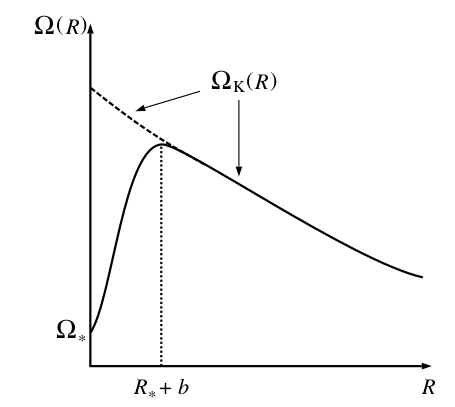
\includegraphics[width=0.7\linewidth]{InnerRegionAngularVelocity}
		\caption{Distribuzione delle velocità angolari $\Omega(R)$ intorno a una stella con $R_{ISCO}=R_\star$ e velocità di rotazione $\Omega_{ISCO}<\Omega_K(R)$}
		\label{fig:InnerRegionAngularVelocity}
	\end{figure}
	
	Trovo che il valore della costante a $R=R_{isco}+b$, esplicitando nell'equazione della conservaizone del momento le definizioni di $G(R)$ ed $\dot{M}$, diventa
	\begin{equation*}
		C=2\pi R_{isco}^3\Sigma v_R\Omega(R_{isco}+b)\vert_{R_{isco}+b}
	\end{equation*}
	e ponendo $\Omega(R_{isco}+b)=\left(\frac{GM}{R_{isco}^3}\right)^{1/2}[1+O(b/R_{isco})]$ diventa, per termini di ordine $b/R_{isco}$:
	\begin{equation}
		C=-\dot{M}(GMR_{isco})^{1/2}
	\end{equation}
	Questa, sostituita nell'equazione della conservazione del momento angolare, con $\Omega=\Omega_K$, porta alla condizione su $\dot{M}$
	\begin{equation}
		\nu\Sigma=\frac{\dot{M}}{3\pi}\left[1-\left(\frac{R_{isco}}{R}\right)^{1/2}\right]
	\end{equation}
	Nel caso in cui valga $b\approx R_{isco}$, l'apporossimazione di disco sottile non sarà più valida da $R=R_{isco}+b$ ad $R_{isco}$ e piuttosto che un anello in cui il materiale rallenta, il disco collasserà ad una conformazione "spessa". Quello che si osserva invece è che $b\ll R_{ISCO}$\footnote{Come dimostrato nella sezione 6.2 del ~\cite{FrankKingRaineAccretionPower}}.
	
	\paragraph{Dissipazione di energia}
	La stazionarietà del disco, nel caso di un corpo centrale che ruota lentamente permette anche di descrivere esplicitamente la dissipazione per unità d'area senza farla dipendere dalla viscosità. Ponendo $\Omega=\Omega_K$, si trova infatti:
	\begin{equation}
		D(R)=\frac{3GM\dot{M}}{8\pi R^3}\left[1-\left(\frac{R_{isco}}{R}\right)^{1/2}\right]
	\end{equation}	
	Con questa funzione siamo in grado di calcolare la luminosità emessa da un anello del disco
	\begin{equation}
		L(R_1,R_2)=2\int_{R_1}^{R_2}D(R)2\pi RdR
	\end{equation}
	Che per $R_1=R_{isco}$ e $R_2\to\infty$ da la luminosità di tutto il disco
	\begin{equation}
		L_{disco}=\frac{3GM\dot{M}}{2R_{isco}}=\frac{1}{2}L_{acc}
	\end{equation}
	
	\paragraph{Struttura verticale del disco}
	In coordinate cilindriche, poiché non mi aspetto nel disco sia presente un meccanismo che permetta del trasporto verticale di materia, lungo questa direzione deve essere mantenuto l'equilibrio idrostatico, ricavabile come parte della componente $z$ dell'equazione di Eulero:
	\begin{equation*}
		\frac{1}{\rho}\frac{\partial P}{\partial z}=\frac{\partial}{\partial z}\left[\frac{GM}{(R^2+z^2)^{1/2}}\right]
	\end{equation*}
	Nell'ipotesi di disco sottile ($z\ll R$) questa diventa
	\begin{equation}
		\frac{1}{\rho}\frac{\partial P}{\partial z}=-\frac{GMz}{R^3}
	\end{equation}
	Se definiamo una scala tipica per le altezze del disco $H$ tale per cui lungo il disco $z\sim H$, possiamo dire che approssimamente $\partial P/\partial z\sim P/H$. Inoltre potrò scrivere $P\sim c_s\rho$.
	Questi fattori insieme comportano che
	\begin{equation}
		H\cong c_s\left(\frac{R}{GM}\right)^{1/2}R
	\end{equation}
	Quindi la condizione di disco sottile $H\ll R$ sarà rispettata se la velocità angolare, che si può dimostrare essere molto vicina a quella kepleriana per il disco sottile, è ampiamente supersonica
	\begin{equation}
		v_\phi(R)=\left(\frac{R}{GM}\right)^{1/2}\gg c_S
	\end{equation}
	Questa è definitivamente una condizione sulla temperatura del disco e per poterla verificare in ogni punto serve un'analisi locale.
	
	Si può dimostrare analogamente che la velocità radiale è ampiamente subsonica per il disco, usando poche definizioni
	\begin{equation}
		v_R\sim\frac{\nu}{R}\sim\alpha c_s\frac{H}{R}\ll c_s
	\end{equation}
	
	\paragraph{Temperatura e Pressione} Abbiamo dimostrato che sotto l'ipotesi di disco sottile, i gradienti in pressione e temperatura come praticamente solo verticali, e possiamo quindi permetterci di tralasciare l'analisi della loro componente radiale (tranne che per la definizione di $D(R)$) e semplificando la descrizione del disco, analizzando
	
	Posso verificare che la condizione di equilibrio idrostatico, per un profilo verticale di temperatura costante, implica che valga
	\begin{equation*}
		\rho(R,z)=\rho_c(R)e^{-z^2/2H^2}
	\end{equation*}
	con $\rho_c$ densità del piano centrale del disco $z=0$.
	
	Quindi assumendo la temperatura centrale del disco sia $T_c(R)=T(R,0)$, posso approssimare la densità centrale di un disco con $\rho=\Sigma/H$, dove $H=Rc_s/v_\phi$ e la velocità del suono è data da $c_s^2=P/\rho$, con la pressione $P$ data dalla somma di pressione di radiazione e gassosa
	\begin{equation}
		P=\frac{\rho\kappa T_c}{\mu m_p}+\frac{4\sigma}{3c}T_c^4
	\end{equation}
	L'equazione della temperatura centrale deve dipendere analogamente da una relazione che leghi il flusso di energia verticale e il tasso di energia generata dai processi di dissipazione viscosi. 
	
	In modo analogo al caso dell'analisi della struttura delle stelle, potremmo chiederci se il tipo di trasporto sia  radiativo o convettivo. Studiando l'adiabaticità del sistema, si osserva che in molti casi il meccanismo di trasporto è quello radiativo. In questo caso il flusso energetico attraverso le superfici del disco vale, a z costante
	\begin{equation}
		F(z)=-\frac{16\sigma T^3}{3\kappa_R\rho}\frac{\partial T}{\partial z}
	\end{equation}
	Con $\kappa_s$ opacità media di Rosseland
	\footnote{Opacità media per un sistema con diversi termini sorgenti di opacità (bb,bf,ff,...)\begin{equation}
																							\frac{1}{k_R}=\frac{\int_0^\infty\frac{1}{k_\nu}\frac{\partial B_\nu(T)}{\partial T}d\nu}{\int_0^\infty\frac{\partial B_\nu(T)}{\partial T}d\nu}
																						\end{equation}}
Questa definizione del flusso corrisponde implicitamente alla condizione che il disco sia \textit{otticamente spesso}, ovvero che valga
	\begin{equation}
		\tau=\rho H\kappa_R(\rho,T_c)=\Sigma\kappa_R\gg 1
	\end{equation}
	Questo perché affinché l'approssimazione a corpo nero sia valida e quindi la radiazione non sia libera di scappare.
	
	Dalla definizione di flusso posso costruire un'equazione del balancio energetico
	\begin{equation}
		\frac{\partial F}{\partial z}=Q^+
	\end{equation}
	Con $Q^+$ densità di energia dissipata tramite processi viscosi, per unità di volume.
	
	Integrando quest'equazione trovo che
	\begin{equation}
		F(H)-F(0)=\int_0^HQ^+(z)dz=D(R)
	\end{equation}
	E poiché $F(z)\sim(4\sigma/3\tau)T^4(z)$, nell'ipotesi che la temperatura superficiale del disco sia molto minore di quella centrale $T_c^4\gg T^4(H)$
	possiamo derivare il risultato
	\begin{equation}
		\frac{4\sigma}{3\tau}T^4_c=D(R)
	\end{equation}
	
	Quindi la struttura del disco che è stato possibile derivare solo usando leggi fondamentali è descritta dalle seguenti espressioni:
	\begin{equation}
	\begin{cases}
		\rho=\Sigma/H\\
		H=c_sR^{3/2}/(GM)^{1/2}\\
		c_s^2=P/\rho\\
		P=\frac{\rho\kappa T_c}{\mu m_p}+\frac{4\sigma}{3c}T_c^4\\
		\frac{4\sigma}{3\tau}T^4_c=\frac{3GM\dot{M}}{8\pi R^3}\left[1-\left(\frac{R_{isco}}{R}\right)^{1/2}\right]\\
		\tau=\rho H\kappa_R(\rho,T_c)=\tau(\Sigma,\rho,T_c)\\
		\nu\Sigma=\frac{\dot{M}}{3\pi}\left[1-\left(\frac{R_{isco}}{R}\right)^{1/2}\right]\\
		\nu=\nu(\rho,T_c,\Sigma,\alpha,...)		
	\end{cases}
	\end{equation}
		
\subsection{La soluzione di Shakura e Sunyaev}
	Per poter risolvere il sistema delle equazioni della struttura del disco stazionario di accrescimento sono necessarie una prescrizione sulla viscosità e una definizione dell'opacità del disco. Nikolai Shakura e Rashid Sunyaev sono riusciti, col loro articolo del 1973 \textit{Black Holes in Binary Systems. Observational Appearance}\footnote{~\cite{ShakuraSunyaev1973}}, a trovare una soluzione semplice ed elegante al problema, con la loro \textit{condizione} $\alpha$:
	\begin{equation}
		\nu=\alpha c_sH
	\end{equation}
Questa è una legge che semplifica la forma dell'equazione della densità superficiale del disco, che ha avuto diversi riscontri sperimentali, ma più di tutto che è riuscita a marginalizzare la gravità della nostra ignoranza riguardo alla natura dei processi viscosi nel disco, parametrizzandoli e riducendo le incognite da studiare ad una sola (la costante $\alpha$). L'altra faccia della medaglia di questa semplificazione nell'analisi delle equazioni e il vero grande problema della teoria dei dischi di accrescimento, come già detto, è che il modello di Shakura e Sunyaev (SeS), non appoggiandosi su osservazioni fisiche, è sterile e non permette di fare previsioni. Siamo solo in grado di confrontare i risultati delle nostre osservazioni con la nostra parametrizzazione del valore che ci aspettiamo $\alpha$ assuma, per provare a capirne la natura.

Per quanto riguarda l'opacità, SeS hanno assunto che la densità $\rho$ e la temeperatura centrale $T_c$ fossero taliche l'opacità media di Rosseland fosse approssimabile con la legge di Kramer
\begin{equation}
	k_R=6.6\times10^{22}\rho T_c^{-7/2}\,cm^2g^{-1}
\end{equation}
e hanno inoltre deciso di trascurare il termine legato alla pressione di radiazione nella formula di $P$.

Con queste ipotesi si ottiene la soluzione del sistema, scritta in termini di $R_{10}=R/(10^10\,cm)$, $M_{1}=M/(M_\odot)$, $\dot{M}_{16}=\dot{M}/(10^16\,g\,sec^{-1})$ e con $f=\left[1-\left(\frac{R_*}{R}\right)^{1/2}\right]^{1/4}$. Poniamo inoltre $\mu=0.615$, valore atteso per un medium completamente ionizzato formato da diversi gas. 

\begin{equation}
	\begin{cases}
		\Sigma=5.2\,\alpha^{-4/5}\dot{M}_{16}^{3/20}M^{1/4}_1R_{10}^{-3/4}f^{14/5}\,g\,cm^{-2}\\
		H=1.7\times10^8\alpha^{-1/10}\dot{M}^{3/20}_{16}M^{-3/8}_1R_{10}^{9/8}f^{3/5}\,cm\\
		\rho=3.1\times10^{-8}\alpha^{-7/10}\dot{M}^{11/20}_{16}M^{5/8}_1R_{10}^{-15/8}f^{11/5}\,g\,cm^{-3}\\
		T_c=1.4\times10^{4}\alpha^{-1/5}\dot{M}^{3/10}_{16}M^{1/4}_1R_{10}^{-3/4}f^{6/5}\,K\\
		\tau=33\,\alpha^{-4/5}\dot{M}^{1/5}_{16}f^{4/5}\\
		\nu=1.8\times10^{14}\alpha^{4/5}\dot{M}^{3/10}_{16}M^{-1/4}_1R_{10}^{3/4}f^{6/5}\,g\,sec^{-1}\\
		v_R=2.7\times10^{14}\alpha^{4/5}\dot{M}^{3/10}_{16}M^{-1/4}_1R_{10}^{-1/4}f^{-14/5}\,cm\,sec^{-1}\\
	\end{cases}
\end{equation}

	Questo sistema di soluzioni rappresenta, per parametri ragionevoli, un disco sottile con $H/R=1.7\times10^8\alpha^{-1/10}\dot{M}^{3/20}_{16}M^{-3/8}_1R_{10}^{1/8}f^{3/5}\,cm$, la cui velocità radiale è subsonica $v_R\sim 0.3\,km\,sec^{-1}$ ($c_s\sim10\,km\,sec^{-1}$) e la cui velocità kepleriana è ampiamente supersonica $v_\phi\sim1000\,km\,sec^{-1}$. Inoltre il disco risulta essere otticamente spesso e praticamente uniforme nella direzione verticale poiché sia $T_c$ che $T(R)$ sono nell'ordine di $\sim\tau^{1/4}\sim2$.

	Anche ipotizzando il nostro valore di $\alpha$ sia mediato verticalmente e, data l'uniformità del sistema, ignorandone quindi la dipendenza da $z$, resta purtroppo completa la nostra ignoranza sulle sue dipendenze da $R$, $M$, $\dot{M}$ e tutte le altre quantità.
	E' evidente come $\alpha$ non compaia nella soluzione con grandi potenze e quindi il suo ordine di grandezza risulti poco rilevante sui risultati delle equazioni di struttura, ma questo significa contemporaneamente che difficilmente potremo stimarne il valore con precisione solo attraverso osservazioni dirette di sistemi binari. 
	
	Se possiamo dire che otteniamo valori realistici dei parametri d'accrescimento dal modello per $\alpha\lesssim1$, sicuramente non avremo elementi validi per capire come si evolva il sistema nel tempo al variare di $R$, $M$ e $\dot{M}$.
	
	Inoltre finché il modello resta valido (e in particolare finché l'approssimazione a legge di Kramer resta valida) il disco può estendersi a raggi piuttosto grandi, finanche a raggiungere l'ordine di grandezza del raggio del lobo di Roche del buco nero e il sistema delle soluzioni implica che anche per $R\sim10^{11}\,cm$, la massa del disco in ogni istante sia
	\begin{equation}
		M_d=2\pi\int^{R_{ext}}_{R_\star}\Sigma RdR\lesssim (10^{-10}M_\odot)\alpha^{-4/5}\dot{M}^{7/10}_16
	\end{equation}
	e quindi, a meno di un paramentro $\alpha$ molto piccolo ($\sim10^{-10}$) sarà sempre molto minore rispetto alla massa del corpo in accrescimento.
	
	Il modello di SeS introduce anche una condizione per poter ignorare l'effetto di auto-gravitazione (\textit{self-gravity}) del disco: affinché questo non si separi in parti auto-gravitanti deve valere
		\begin{equation}
			\rho\ll M/R^3
		\end{equation}
	condizione rispettata a meno che $\alpha$ sia molto piccolo ($\sim10^{-10}$).
	
	\paragraph{Regioni dominate da pressione di radiazione}
	Per quanto riguarda l'ipotesi che l'opacità sia regolata dalla legge di Kramer, possiamo osservare che per il nostro sistema delle soluzioni l'opacità è indipendente da $\alpha$ ed è espressa come
	\begin{equation}
		k_R(Kramer)=\tau/\Sigma=6.3\dot{M}^{-1/2}_{16}M^{-1/4}_1R^{3/4}_{10}f^{-2}
	\end{equation}
	Se per un gas completamente ionizzato a $T\gtrsim10^4\,K$ il termine dominante di opacità deriva dallo scattering elettronico con $k_R(scat. elett.)\cong\sigma_T/m_p\cong0.4\,cm^2\,g^{-1}$, l'opacità regolata da Kramer deve essere dominante per	
	\begin{equation}
		R\gtrsim R_K=2.5\times10^8\dot{M}^{2/3}_{16}M^{1/3}_1f^{8/3}\,cm
	\end{equation}
	Questo raggio, per tassi di accrescimento ragionevoli, è molto minore del raggio di una nana bianca, ma non meno dell'ultima orbita stabile di un buco nero.
	
	Poiché in prossimità del bordo esterno del disco ($R_{10}\sim1$) ci aspettiamo $T_c$ possa scendere molto al di sotto dei $10^4\,K$, per cui è valida la descrizione dell'opacità con la legge di Kramer come risultato della ricombinazione dell'idrogeno, dobbiamo analizzare il comportamento dell'opacità in queste regioni.
	
	Il rapporto tra la pressione radiativa e quella gassosa vale sul disco
	\begin{equation}
		\frac{P_r}{P_g}=2.8\times10^{-3}\alpha^{1/10}\dot{M}^{7/10}_{16}R^{-3/8}_{10}f^{7/5}
	\end{equation}
ed è molto piccolo per le regioni dominate dall'opacità di Kramer ($R\gtrsim R_K$), dove quindi vale la soluzione di SeS.
	
	Al contrario nelle regioni con $R\lesssim R_K$ l'opacità è dominata dallo scattering elettronico, anche se permane la condizione $P_r\ll P_g$. In queste regioni, poiché l'opacità non è più generata dai processi inversi a quelli radiativi, lo spettro di emissione non sarà simile a quello di corpo nero, ma piuù schiacciato.
	
	Dalla formula del rapporto dei raggi si può osservare che la pressione di radiazione ha un'importanza crescente rispetto a quella gassosa per raggi decrescenti. Shakura e Sunyaev hanno osservato come questa tendenza si intensifichi e continui nella regione di scattering elettronico e che la pressione radiativa supera quella gassosa nella regione con
	\begin{equation}
		R\lesssim R_P=24\alpha^{2/21}\dot{M}^{16/21}_{16}M^{-3/21}_1f^{4/21}\,km
	\end{equation}
	Questo raggio è oltre la superfice dei corpi in accrescimento solo nel caso di stelle a neutroni e buchi neri e per tassi di accrescimento $\dot{M}_{16}\gtrsim 1$.
	
	Date le deboli dipendenze dal parametro $\alpha$ nelle equazioni del rapporto tra le pressioni, $R_K$ e $R_P$, posso costruire un diagramma che rappresenti ragionevolmente le diverse regioni del disco\footnote{Immagine da ~\cite{FrankKingRaineAccretionPower}}
	
	\begin{figure}[H]
		\centering
		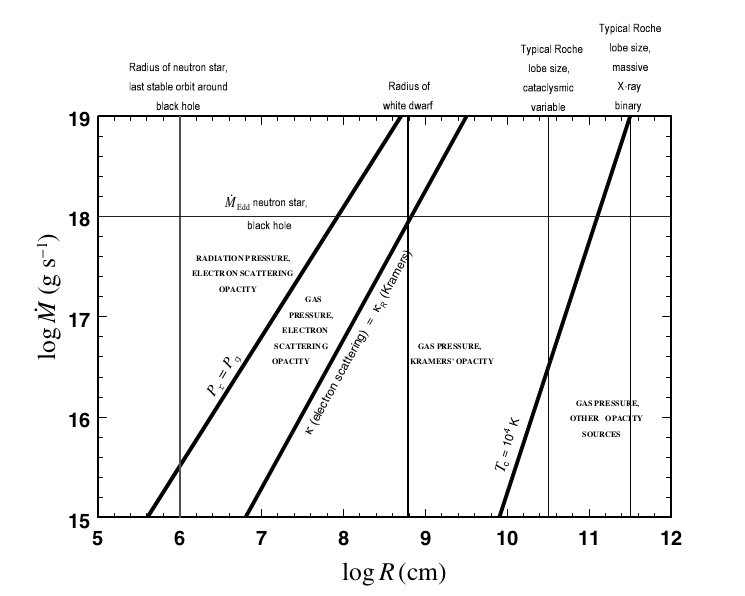
\includegraphics[width=1\linewidth]{MappaPressione}
		\caption{Mappa dei regimi di pressione in un disco stazionario di Shakura e Sunyaev}
		\label{fig:MappaPressione}
	\end{figure}
	
	E' possibile derivare un importante risultato relativo alle regioni dominate da pressione di radiazione relativo all'altezza del disco a partire dal sistema delle equazioni per un disco stazionario.
	
	In particolare dalle formule per $H$, $c_s$, $P$ e $T_c$ e trascurando i termini relativi alla pressione gassosa si trova che la velocità del suono nel disco vale
	\begin{equation*}
		c_s^2=\frac{3GM\dot{M}\tau}{8\pi R^3\rho c}\left[1-\left(\frac{R_{ISCO}}{R}\right)^{1/2}\right]
	\end{equation*}
	E poiché in queste regioni l'opacità è dovuta allo scattering elettronico, la profondità ottica sarà descritta da
	\begin{equation*}
		\tau=\Sigma\kappa_R(e.s.)\cong\rho H\sigma_T/m_p
	\end{equation*}
	Quindi sostituendo questi risultati nella formula per l'altezza locale si trova che
	\begin{equation}
		H\cong\frac{3\sigma_T\dot{M}}{9\pi m_pc}\left[1-\left(\frac{R_{ISCO}}{R}\right)^{1/2}\right]
	\end{equation}
		 
	Quindi possiamo dire che l'altezza del disco nelle regioni supportate da pressione di radiazione è circa indipendente dal raggio. Questo è legato al fatto che le forze di pressione $\sim T_c^4\sim M\dot{M}R^{-3}$ sono opposte alla componente verticale della gravità $\propto MHR^{-3}$.
	
	Posso legare questa formula dell'altezza del disco al limite di Eddington
	\begin{equation*}
		\dot{M}=\frac{4\pi GMm_pc^3}{\sigma_T \eta}
	\end{equation*}
	Che la fa diventare quindi una condizione sul tasso di accrescimento perché sia mantenuta la struttura sottile del disco
	\begin{equation}
		H\cong\frac{3R_{ISCO}}{4\eta}\frac{\dot{M}}{\dot{M}_{crit}}\left[1-\left(\frac{R_{ISCO}}{R}\right)^{1/2}\right]
	\end{equation}
	Col loro modello SeS sono stati in grado di dimostrare quindi come l'accrescimento possa produrre una luminosità superiore a quella limite di Eddington, ma hanno anche dedotto che in queste condizioni la pressione radiativa avrebbe espulso la materia in eccesso, cosa che si è osservata accadere  nelle sorgenti x ultra-luminose (ULXs).
	
	Comunque questo non è ovviamente l'unico caso in cui il disco smetta di essere sottile, per esempio anche una temperatura centrale molto superiore di quella di un corpo nero potrerebbe a risultati simili.
	
\subsection{Spettro di emissione}

	Poiché abbiamo prescritto che il disco sia otticamente spesso nella direzione $z$, per cui mi aspetto ogni elemento del disco irradi come un corpo nero e quindi con temperatura $T(R)$ tale che
	\begin{equation}
		\sigma T^4(R)=D(R)
	\end{equation}
	Da cui ricavo, utilizzando la definizione di $D(R)$
	\begin{equation}
		T(R)=\left\{\frac{3GM\dot{M}}{8\pi R^3\sigma}\left[1-\left(\frac{R_{ISCO}}{R}\right)^{1/2}\right]\right\}^{1/4}
	\end{equation}
	Posso trattare questa temperatura come un valore efficace del disco, da cui ricavare un valore dell'intensità per frequenza emessa da ogni elemento d'area del disco
	\begin{equation}
		I_\nu=B_\nu[T(R)]=\frac{2h\nu^3}{c^2(e^{h\nu/kT(R)}-1)}
	\end{equation}
	Questo risultato non tiene conto dell'effetto di redistribuzione dell'intensità rispetto alle frequenze prodotto dall'atmosfera otticamente sottile del disco.
	
	Per un osservatore il cui angolo di vista abbia un angolo $i$ rispetto alla normale al piano del disco, posso definire il flusso per frequenza come
	\begin{equation}
		F_\nu=\frac{2\pi \cos{i}}{D^2}\int^{R_{ext}}_{R_{ISCO}}RI_\nu dR=\frac{4\pi h\nu^3\cos{i}}{c^2D^2}\int^{R_{ext}}_{R_{ISCO}}\frac{R}{e^{h\nu/kT(R)}-1}dR
	\end{equation}

	Questo flusso è indipendente dalla viscosità per le ipotesi di corpo nero e disco stazionario.
	
	\begin{figure}[H]
		\centering
		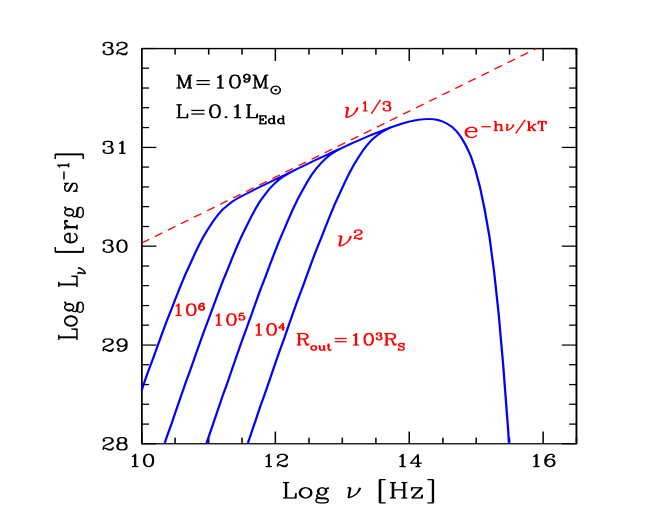
\includegraphics[width=0.7\linewidth]{SpettroDiscoGhisellini}
		\caption{Spettro di un disco di accrescimento nel caso di un buco nero supermassiccio}
		\label{fig:SpettroDiscoGhisellini}
	\end{figure}	

	Se rappresento lo spettro in un sistema bilogaritmico\footnote{Immagine da ~\cite{GhiselliniRadiativi}} posso apprezzare il comportamento asintotico del flusso, che dipende da quello della plankiana
	\begin{equation}
		F_\nu\propto\begin{cases}
						\nu^2 & \nu\ll kT(R_{ext})/h \textit{ "regione di Rayleigh-Jeans"}\\
						\nu^{1/3} & kT(R_{ISCO})/h\ll\nu\ll kT(R_{ext})/h\\
						e^{-h\nu/kT} & \nu\gg kT(R_{ISCO})/h \textit{ "regione di Wien"}						
					\end{cases}
	\end{equation}
	Il comportamento a frequenze intermedie $F_\nu\propto\nu^{1/3}$ è considerato caratteristico dei dischi di accrescimento e la lunghezza della regione con quella pendenza dipende dalla differenza di temperatura tra il bordo interno e quello del disco. Se $T(R_{ISCO})\cong T(R_{ext})$ lo spettro di emissione del disco si avvicina sempre più a quello di un corpo nero.

	\emph{La temperatura efficace di un disco sottile stazionario scala come $T(R)\propto R^{-3/4}$, indipendetemente dal meccanismo con cui il gas perde momento angolare...\\Nel caso dell'accrescimento intorno a un buco nero da parte di una stella ordinaria è plausibile che la radiazione sia emessa sotto forma di bremmstrahlung, per via della ridotta zona effettiva di emissione, con temperatura $T\gtrsim10^7\,K$ e poiché lo spettro è irradiato principalmente negli X. La radiazione proviene quasi completamente dal disco circa con una legge di potenza (\textit{power law}).\\Se il flusso di materia è così grande che la pressione di radazione prevenga l'accrescimento stazionario o così bassa che l'energia gravitazionale non possa venire irradiata in modo efficente, ci si aspettano dei "flaring", con il buco nero che alterna l'accrescimento all'espulsione di materia dalla sua regione più prossima.}
	
\newpage
\section{Evoluzione temporale dei dischi e instabilità}
\subsection{Instabilità termica e viscosa}
\subsection{Considerazioni sull'espressione della viscosità}
\subsection{Spettro di emissione}
\newpage
\section{Conclusione}

\newpage
\renewcommand{\bibpreamble}{Per regioni di coerenza interna al testo e di visione ordinata degli argomenti, ho cercato di affrontarli seguendo il più delle volte la traccia e le argomentazioni come sono presentatate sul testo di \textit{Frank, King e Raine}~\cite{FrankKingRaineAccretionPower}, manuale di riferimento per quanto riguarda le teorie dell'accrescimento.
	
	Sono stati fondamentali anche alcune  \textit{review} di \textit{King}~\cite{King2012} e \textit{Pringle}~\cite{Pringle1981}, che sintetizzano efficacemente l'argomento dell'accrescimento e permettono di avere una visione di insieme dei risultati ottenuti.
	
	E' stato fondamentale per la mia comprensione dello sviluppo delle teorie, l'analisi e la lettura degli articoli originali sui modelli di disco di accrescimento intorno ai corpi compatti.
	Ho lavorato quindi anche con gli articoli seminali di \textit{Pringle}, \textit{Reese}, \textit{Shakura}, \textit{Sunyaev} e \textit{Pacholczyk}~\cite{PringleReese1972}~\cite{PringleReesePacholczyk1973}~\cite{ShakuraSunyaev1973} e la splendida analisi del lavoro nella fondazione della teoria di accrescimento di Zeldovich svolta da Shakura quest'anno~\cite{ShakuraZeldovich2018}.
	
	Per quanto riguarda in particolare l'argomento della tesi, ovvero l'instabilità nelle regioni dominate dalla pressione radiativa nel modello del disco di accrescimento, ho fatto riferimento al primissimo lavoro a riguardo di \textit{Lightman} ed \textit{Eardley}~\cite{LightmanEardley1974} e ad articoli successivi che estendono, propongono alternative, ne analizzanoi risultati o li computano. Questi sono stati scritti da \textit{Shakura} e \textit{Sunyaev}~\cite{ShakuraSunyaev1976}, \textit{Shapiro} con gli stessi \textit{Lightman} ed \textit{Eardley}~\cite{ShapiroLightmanEardley1976}, \textit{Taam} e \textit{Lin}~\cite{TaamLin1984} e \textit{Teresi}, \textit{Molteni} e \textit{Toscano}~\cite{TeresiMolteniToscano2004}.
	
	Per tutti gli aspetti non strettamente legati all'accrescimento ho fatto riferimento a tre manuali: il \textit{Maoz}~\cite{MaozNutshell} e il \textit{Prialnik} ~\cite{PrialnikStellarStructureEvolution} per i cenni sulla struttura dei corpi compatti e il \textit{Ghisellini}~\cite{GhiselliniRadiativi} per quanto riguarda i processi radiativi.}

\begin{thebibliography}{9}
	\bibitem{FrankKingRaineAccretionPower} 
	J. Frank, A. King, D. Raine
	"Accretion Power in Astrophysics"\\
	\textit{Cambridge University Press}, 2002 (III ed.)
	
	\bibitem{King2012} 
	A. King 
	"Accretion Disc Theory since Shakura and Sunyaev"\\
	\textit{arXiv}: 1201.2060v1\\
	\textit{to appear in proceedings of 'The Golden Age of Cataclysmic Variables', Memorie Società Astronomica Italiana, 2012 (F. Giovannelli and L. Sabau-Graziati eds.)}
	
	\bibitem{GhiselliniRadiativi} 
	G. Ghisellini
	"Radiative Processes in High Energy Astrophysics"\\
	\textit{Springer}, 2013
	
	\bibitem{LightmanEardley1974} 
	A. P. Lightman, D. M. Eardley 
	"Black Holes in Binary Systems: Instability of Fisk Accretion"\\
	\textit{Astrop. Journal} 187, L1-L3, 1974 January 1
	
	\bibitem{MaozNutshell} 
	D. Maoz
	"Astrophysics in a nutshell"\\
	\textit{Princeton University Press}, 2007
	
	\bibitem{PrialnikStellarStructureEvolution} 
	D. Prialnik
	"An Introduction to the Theory of Stellar Structure and Evolution"\\
	\textit{Cambridge University Press}, 2000
	
	\bibitem{Pringle1981} 
	J. E. Pringle 
	"Accretion Discs in Astrophysics"\\
	\textit{Ann. Rev. Astron. Astrphys.} 1981, 19:137-62
	
	\bibitem{PringleReese1972} 
	J. E. Pringle, M. J. Rees
	"Accretion Discs Model for Compact X-Ray Sources"\\
	\textit{Astron. \& Astrphys.} 21, 1-9 (1972)
	
	\bibitem{PringleReesePacholczyk1973} 
	J. E. Pringle, M. J. Rees, A. G. Pacholczyk
	"Accretion onto Massive Black Holes"\\
	\textit{Astron. \& Astrphys.} 29, 179-184 (1973)
	
	\bibitem{ShakuraSunyaev1973}
	N. I. Shakura, R. A. Sumyaev 
	"Black Holes in Binary Systems. Observational Appearance"\\
	\textit{Astron. \& Astrophys.} 24, 337-355 (1973)
	
	\bibitem{ShakuraSunyaev1976}
	N. I. Shakura, R. A. Sumyaev 
	"A Theory of the Instability of Disk Accretion on to Black Holes and the Variability of Binary X-Ray Sources, Galactic Nuclei and Quasars"\\
	\textit{Mon. Not. R. astr. Soc.} (1976) 175, 613-632
	
	\bibitem{ShakuraZeldovich2018}
	N. I. Shakura
	"Ya. B. Zeldovich and foundation of the accretion theory"\\
	\textit{arXiv}: 1809.1137v1
	
	\bibitem{ShapiroLightmanEardley1976} 
	S. L. Shapiro, A. P. Lightman, D. M. Eardley 
	"A Two-Temperature Disk Model for Cygnus X-1 Structure and Spectrum"\\
	\textit{Astrop. Journal} 187-199, 1976 February 15
	
	\bibitem{TaamLin1984} 
	R. E. Taam, D. N. C. Lin 
	"The Evolution of the Inner Regions of Viscous Accretion Disks Surrounding Neutron Stars"\\
	\textit{Astrop. Journal} 287, 761-768 1984 December 15
	
	\bibitem{TeresiMolteniToscano2004} 
	V. Teresi, D. Molteni, E. Toscano 
	"SPH Simulations of Shakura-Sunyaev Instability at Intermediate Accretion Rates"\\
	\textit{Mon. Not. R. Astron. Soc.} 348, 361-367 (2004)
\end{thebibliography}

\end{document}
